%% Journal manuscript carved from the B.Sc. thesis
%% "Conformalized Discrete-Time Hazard Modeling for Multi-Horizon Handover Forecasting in Cellular Networks".
%% Target: Computer Communications / Computer Networks (Elsevier). Build: pdflatex main && pdflatex main
%% For the single-column review layout most Elsevier submission systems ask for, swap the class line:
%%   \documentclass[preprint,review,12pt]{elsarticle}
\documentclass[preprint,review,12pt]{elsarticle}\usepackage{lineno}\linenumbers

\usepackage{amsmath,amssymb}
\usepackage{graphicx}
\usepackage{booktabs}
\usepackage{tabularx}
\usepackage{multirow}
\usepackage{xcolor}
\usepackage{listings}
\usepackage[hidelinks]{hyperref}
\usepackage{microtype}

\lstset{basicstyle=\ttfamily\footnotesize,columns=fullflexible,breaklines=true,
        frame=single,framerule=0.3pt,xleftmargin=2pt,xrightmargin=2pt,
        keywordstyle=\bfseries,language=Python,showstringspaces=false}

\newcommand{\x}{$\times$}

\journal{Computer Communications}

\begin{document}

\begin{frontmatter}

\title{Timestamp-Alignment Leakage in Drive-Test Handover Prediction: Quantification, Mitigation, and Blind Second-Operator Validation}

\author[iut]{Saadman Sakib\corref{cor}}
\ead{saadmansakib21@iut-dhaka.edu}
\author[iut]{Adhnan Kalim\corref{cor}}
\ead{adhnankalim@iut-dhaka.edu}
\author[iut]{Evan Ashfaque\corref{cor}}
\ead{evanashfaque@iut-dhaka.edu}
\author[iut]{Mohammad Tawhid Kawser}
\cortext[cor]{Corresponding authors.}
\affiliation[iut]{organization={Department of Electrical and Electronic Engineering, Islamic University of Technology (IUT)},
            addressline={Board Bazar},
            city={Gazipur},
            postcode={1704},
            country={Bangladesh}}

\begin{abstract}
Learned handover predictors are often trained on one-hertz drive-test exports and report high scores. We show that a property of the export, not of the network or learner, can produce much of that score. In four drive-test campaigns on a commercial LTE network (10,260 one-hertz samples, 938 handover commands decoded from RRC signalling), the export row stamped in the second before a handover command already carries the post-handover serving cell in 76\% of handovers, against 16\% one row earlier. Lagging every export feature by one row moves the one-second area under the precision--recall curve (AUPRC) of the same fixed-parameter model from 0.604 to 0.156, a 3.9-fold inflation; 94\% of the fall comes from serving-cell radio scalars that change their referent when the serving cell flips. End-of-second downsampling of a native-rate public corpus from the same tool (4,712 handovers, three operators) reproduces the defect (93\%), and start-of-second downsampling removes it (4\%). A capture on a second operator, recorded after the pipeline was frozen and blind to the repair, replicates both findings: 67\% contamination and a 4.3-fold inflation. With the leak removed and whole campaigns held out, an exploratory evaluation gives a one-second AUPRC of 0.169 against a 6.8\% prevalence floor, and the splitting protocol reorders the learners: random-row splitting inflates gradient-boosted trees by 49\% and a linear model by 8\%. On the blind operator the predictive level transferred but the ranking of learners did not. The audit takes a few lines of code and is released with the pipeline.
\end{abstract}

\begin{highlights}
\item One-hertz drive-test rows carry the post-handover cell before the handover command.
\item Ignoring this inflates one-second handover-prediction AUPRC about four-fold.
\item Serving-cell radio scalars, not cell identifiers, carry 94\% of the leak.
\item Splitting protocol reorders learner rankings, not just their scores.
\item The leak replicates blind on a second operator; learner rankings do not.
\end{highlights}

\begin{keyword}
Handover prediction \sep Data leakage \sep Drive test \sep LTE \sep RRC signalling \sep Evaluation protocol \sep Discrete-time survival analysis
\end{keyword}

\end{frontmatter}

%% =====================================================================
\section{Introduction}
\label{sec:intro}

Long Term Evolution (LTE) networks hand a connected user from one cell to another mostly through Event~A3: the user equipment (UE) reports when a neighbour cell has become stronger than the serving cell by a configured offset for a configured time-to-trigger (TTT), and the network then issues the handover command~\cite{ref1}. The rule is reactive by construction, which is why a large body of recent work tries to forecast the handover, the radio-link failure or the next serving cell from measurements the handset already reports~\cite{ref7,ref8,ref9,ref54}. Many of those predictors are trained on the tabular exports of commercial drive-test tools, which summarise radio state on a one-hertz grid, and many report scores that would make proactive mobility management straightforward.

This paper is about a reason to distrust such scores that has nothing to do with the learner. A one-hertz export row has to summarise a second, and a handover executes in tens of milliseconds. If the exporter writes the state at the end of the second into a row stamped at its start, the row stamped just before a handover command already shows the cell the handset is about to move to. Every feature in that row looks causal: it carries no future label, it is not a future row, and grouped splitting does not remove it, because the leak sits inside the row rather than between rows. In the taxonomy of Kaufman et al.~\cite{ref36} it is leakage in the training examples, the class that is hardest to catch because every syntactic check passes. Kapoor and Narayanan~\cite{ref56} document how often leakage of this general kind propagates through machine-learning-based science. What we add is a specific measurement mechanism, its size on handover prediction, and a procedure for detecting it against the event clock that RRC signalling provides.

We found the defect in our own work. A first version of this study reported a one-second AUPRC of 0.60 on four drive-test campaigns; an audit of the export against decoded RRC timestamps showed that most of that figure came from the row alignment. The study was then rebuilt around the audit, and a fifth capture on a second operator was recorded after the pipeline was frozen, to test the methodological findings on data that had played no part in deriving them.

The contributions are the following.
\begin{enumerate}
\item \emph{An alignment audit and its mechanism.} In 76\% of 938 handovers the export row stamped before the command already carries the target cell, against 16\% one row earlier (Section~\ref{sec:audit}). A margin model of end-of-second aggregation predicts which handovers are contaminated, and two external corpora support it: end-of-second downsampling of native-rate XCAL data from three US operators reproduces the defect (93\%) and start-of-second downsampling removes it (4\%), while a tool that samples rather than aggregates shows no aggregation step.
\item \emph{The cost of the leak, and where it lives.} On the same model, folds and hyper-parameters, lagging every export feature by one row moves one-second AUPRC from 0.604 to 0.156. Lagging the 31 neighbour and A3-gap columns alone changes almost nothing; lagging the 56 serving-cell radio scalars accounts for 94\% of the fall (Section~\ref{sec:cost}). The columns to distrust are the ones defined relative to the serving-cell assignment.
\item \emph{The protocol reorders the leaderboard.} With features, hyper-parameters and seeds held fixed, random-row splitting inflates gradient-boosted trees by 49\% over leave-one-campaign-out and a linear model by 8\%, so the protocol used in most of the comparator literature would name a different winner on the same data (Section~\ref{sec:ladder}).
\item \emph{An honest reference level.} With the leak removed and whole campaigns held out, the next handover is predictable only modestly: AUPRC 0.169 at one second against a 6.8\% floor, 33\% of commands detected at 169 false alarms per hour (Section~\ref{sec:level}). A discrete-time hazard formulation keeps the five horizons coherent from a single fit for any learner.
\item \emph{A blind second-operator test.} On a capture blind to every pipeline decision, both methodological findings replicate (67\% contamination; 4.3-fold inflation), the predictive level transfers, and the ranking of learners does not (Section~\ref{sec:blind}).
\end{enumerate}

Two scope statements frame everything that follows. The four development campaigns are exploratory evidence: the alignment repair was derived with all four in view, so none of them, the held-out highway campaign included, is blind to pipeline design. And the paper does not offer a deployable predictor. Its contribution is the measurement and evaluation framework, and the reference numbers that framework produces.

%% =====================================================================
\section{Related work}
\label{sec:related}

\paragraph{Measurement of mobility management} Measurement studies decode RRC signalling from diagnostic interfaces to recover deployed mobility configurations and their consequences~\cite{ref3,ref4,ref5,ref41}. Deng et al.~\cite{ref3} and Ghoshal et al.~\cite{ref4} characterise configuration diversity across operators; Hassan et al.~\cite{ref5} dissect 5G mobility management and include a handover-prediction component. Handovers also have measurable consequences for transport and for ping-pong behaviour~\cite{ref6,ref14}. This literature establishes signalling as ground truth, but it does not join that ground truth to the evaluation of learned predictors, and it does not examine the alignment between a tool's tabular export and its own event clock.

\paragraph{Learned handover prediction and its evaluation} To situate the protocol used here, we screened 108 publications from 2020--2026 and audited the 22 that present a learned or analytical model predicting handover, radio-link failure, blockage or next-cell occupancy; 16 of them are direct learned forecasters. Table~\ref{tab:audit} summarises the audit; the audited forecasters include~\cite{ref15,ref45,ref46,ref54,ref57,ref58,ref59,ref60,ref61,ref62,ref63,ref64,ref65,ref66,ref67,ref68,ref69,ref70}, and the per-paper extraction is part of the released archive. Of the 16, none holds out a drive, session or route; nine state no split protocol at all; seven report accuracy on tasks whose positive prevalence lies between 0.86\% and 11\%, where a constant negative prediction scores 89--99\%; none reports calibration or warning lead time; and none states how its measurement timestamps are aligned with its event clock. The closest comparator on real network measurements, Dzaferagic et al.~\cite{ref54}, forecasts handovers on an O-RAN deployment from one-second samples, sweeps the horizon and weighs prediction against the cost of acting on it; it states a 60/20/20 allocation but not the split unit, and no alignment rule. Recent sequence-model studies on drive-test traces~\cite{ref45,ref46} are likewise silent on alignment. The audit concerns sixteen recent learned forecasters, not the field as a whole, and its search was assembled from topic threads rather than one fixed database query.

\begin{table}[t]
\centering
\caption{Protocol audit of the 16 direct learned forecasters among 22 audited models (2020--2026), against this work.}
\label{tab:audit}
\footnotesize
\begin{tabularx}{\linewidth}{X c l}
\toprule
\textbf{Protocol property} & \textbf{Of 16} & \textbf{This work} \\
\midrule
Holds out a drive, session or route & 0 & Campaign hold-out \\
Any split coarser than a random row & 3 & Four protocols compared \\
States a split protocol & 7 & Yes \\
Prevalence-aware ranking metric & 2 & AUPRC with floor \\
Reports calibration & 0 & ECE and Brier \\
Reports lead time or false alarms per hour & 0 & Both \\
Headline accuracy on an imbalanced task & 7 & Never \\
States export--event-clock alignment & 0 & Audited \\
\bottomrule
\end{tabularx}
\end{table}

\paragraph{Leakage and dependent data} Kaufman et al.~\cite{ref36} formalise leakage and its detection, Kapoor and Narayanan~\cite{ref56} show its reach across applied machine learning, and Roberts et al.~\cite{ref35} show that random cross-validation on temporally or spatially structured data is optimistic and recommend blocking. Our protocol ladder applies that argument to drive-test data and measures it; our alignment audit concerns a mechanism none of these works addresses, because it arises inside a single row of an instrument's export.

\paragraph{Time-to-event formulations and distribution-free calibration} Cell-sojourn and handover-rate analyses derive marginal time-to-event laws under assumed mobility and geometry~\cite{ref42,ref43,ref44}. Discrete-time survival models conditioned on covariates are standard in event-history analysis~\cite{ref48,ref49,ref50} and have deep-learning variants~\cite{ref16,ref17}; conformal methods have also been combined with survival analysis~\cite{ref18}. Conformal risk control~\cite{ref21,ref22} provides finite-sample guarantees on monotone losses under exchangeability, and conformal calibration has been advocated for wireless AI~\cite{ref19,ref20} and applied to channel prediction~\cite{ref55}. We use the hazard formulation for coherence across horizons and conformal risk control only as an empirical calibration diagnostic, because campaigns separated by covariate shift are not exchangeable~\cite{ref51,ref52}; adaptive conformal inference~\cite{ref53} controls a long-run average instead and was not evaluated here.

%% =====================================================================
\section{Measurement corpus and ground truth}
\label{sec:corpus}

\paragraph{Instrumentation} All captures used one commercial drive-test handset running Accuver XCAL, which produces two synchronised outputs from the chipset diagnostic interface: a tabular radio export on a one-hertz grid (serving-cell PCI and EARFCN, RSRP, RSRQ, SINR, CQI, GPS speed and heading) and a decoded control-plane log with millisecond timestamps. The ground-truth event is the decoded \texttt{RRCConnectionReconfiguration} carrying \texttt{mobilityControlInfo}, that is, the handover command; all 957 decoded commands carry a matched \texttt{RRCConnectionReconfigurationComplete}. Neighbour measurements are not populated in the periodic export, so they are recovered from \texttt{MeasurementReport} messages and projected onto the grid with a backward-looking hold of at most 3~s.

\paragraph{Signalling decoding} Resolving a report to the event that triggered it requires replaying the UE's \texttt{VarMeasConfig} as a timeline, applying the removal lists, the measId swap of TS~36.331 clause~5.5.6.1 on inter-frequency handover, and the release on leaving RRC\_CONNECTED~\cite{ref1}. A flat union of configuration fragments classified 99.4\% of reports as A3; the timeline classifies 39--45\%. The neighbour parser also respects the optionality of RSRQ in \texttt{measResultListEUTRA}: 25--36\% of neighbour entries on the development operator, and 98\% on the second operator, carry RSRP only. Both corrections were made from the message grammar without reference to any model output.

\begin{figure}[t]
\centering
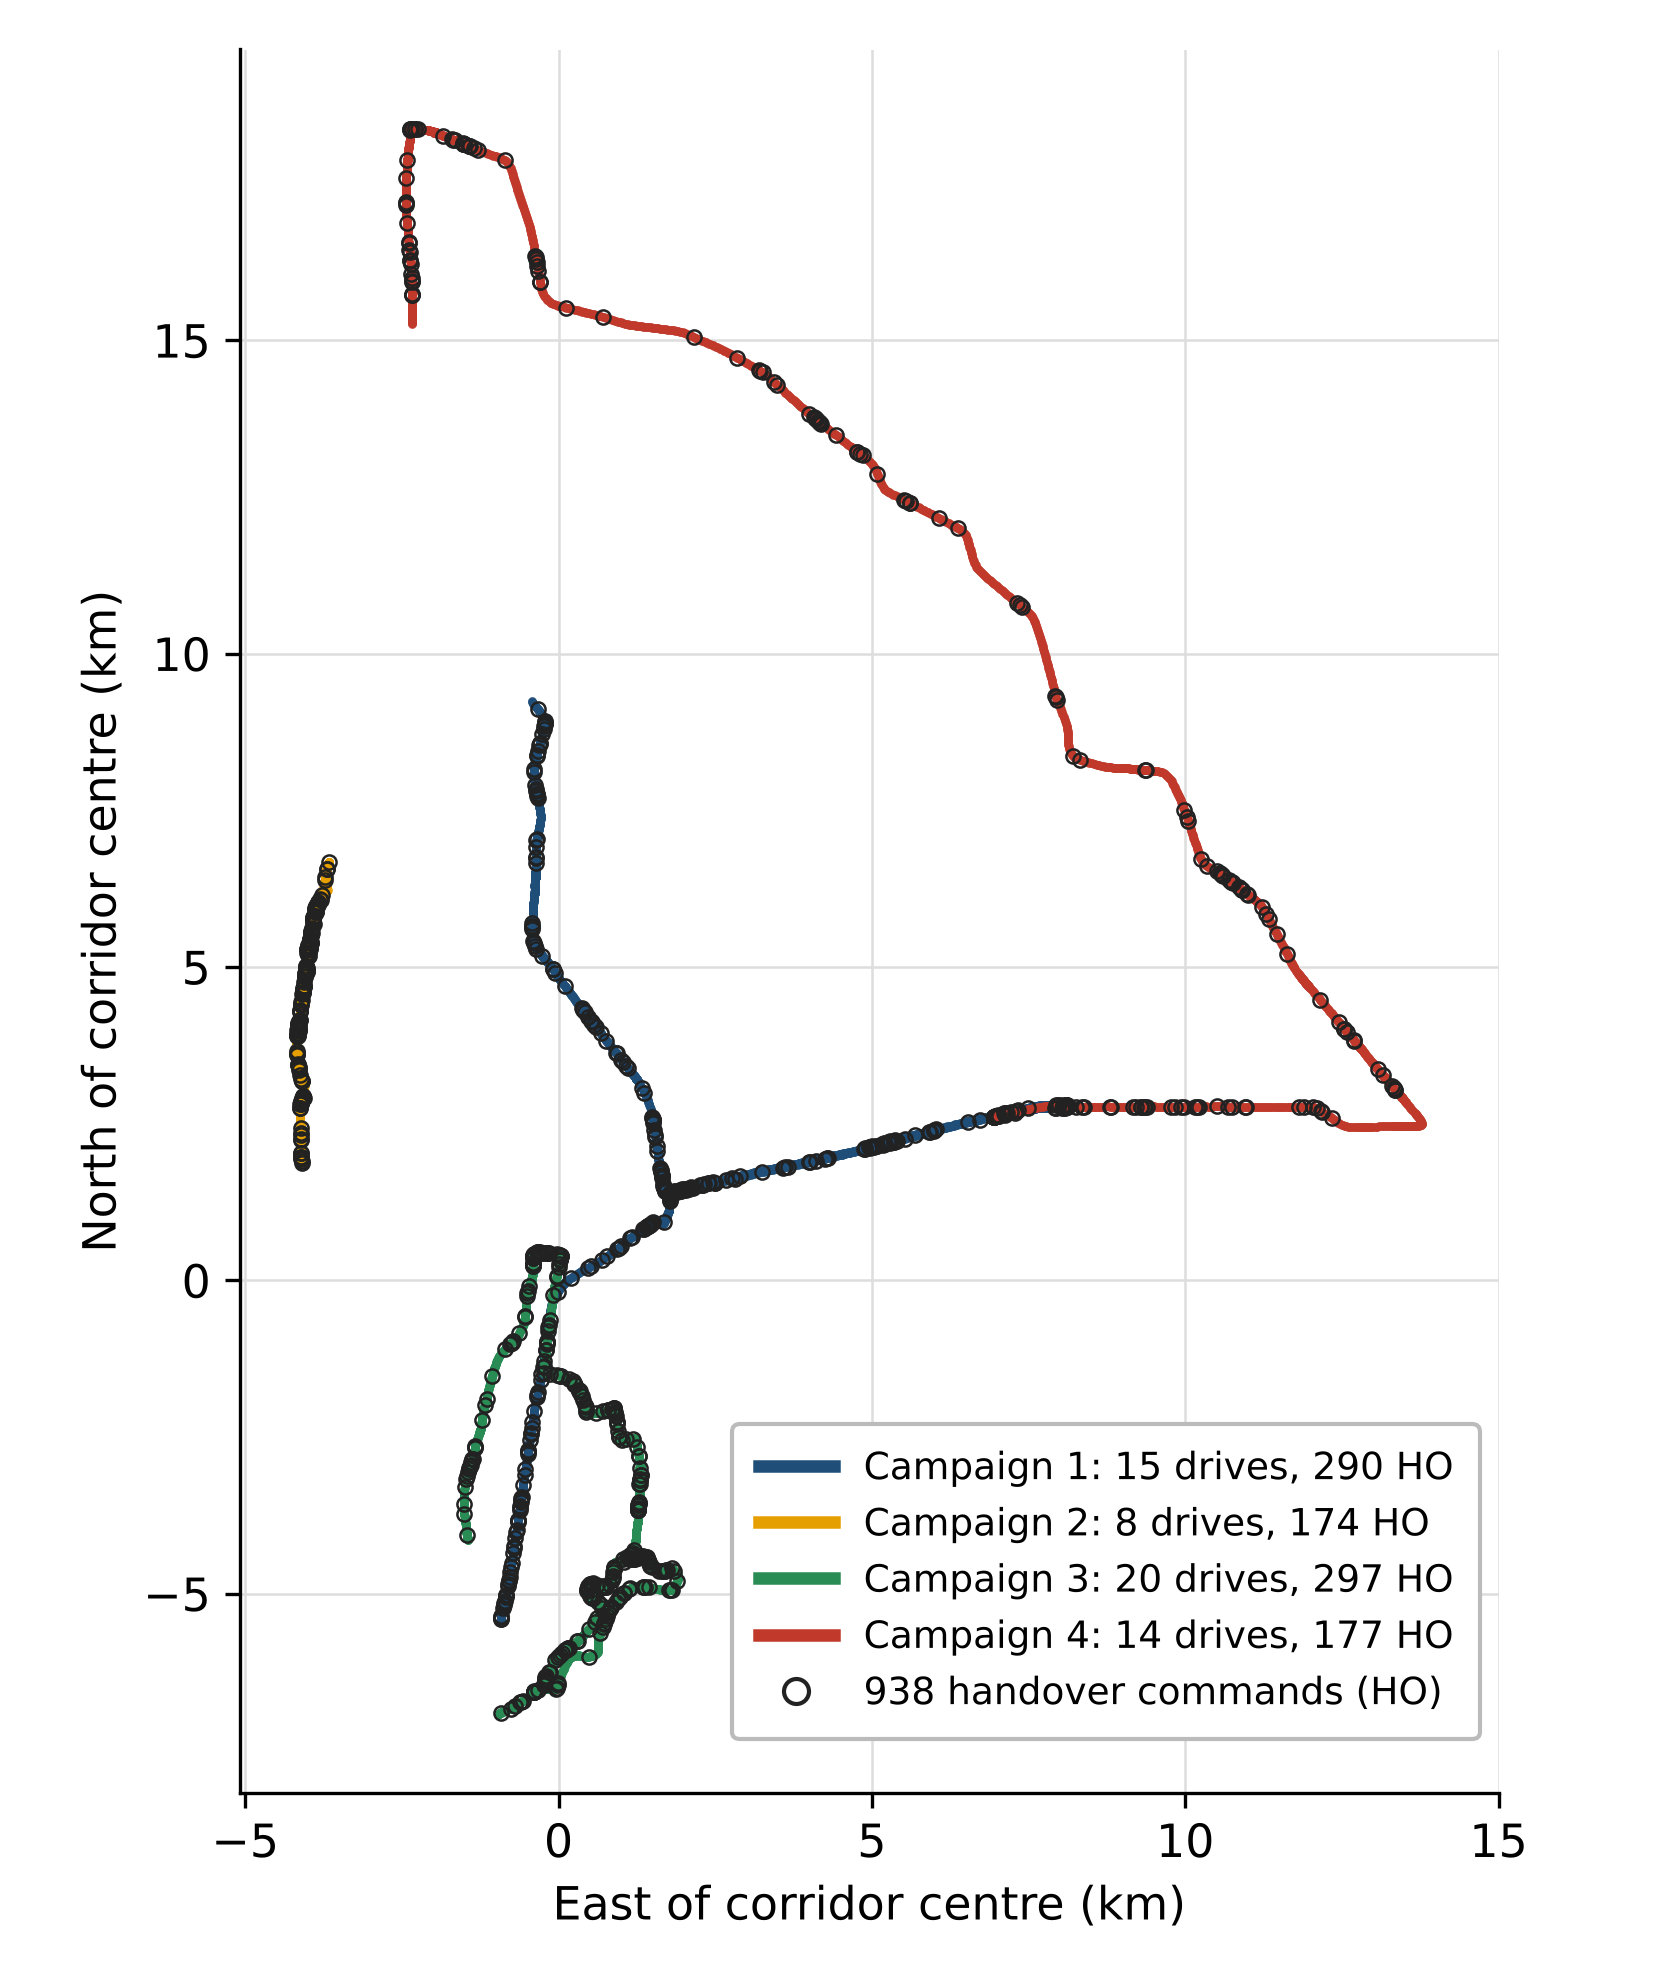
\includegraphics[width=0.82\linewidth]{figures/fig03_map_routes.png}
\caption{Routes of the four development campaigns (operator~A), Dhaka urban corridors and the Uttara--Gazipur highway. Open circles mark the 938 quality-controlled handover commands (HO); the legend gives the drives and commands per campaign.}
\label{fig:map}
\end{figure}

\paragraph{Campaigns} Four campaigns were driven on one commercial LTE operator (operator~A) in Dhaka and Gazipur in September 2026: an urban arterial road, an urban loop, a dense urban area, and the Uttara--Gazipur highway (Fig.~\ref{fig:map}, Table~\ref{tab:corpus}). Each is one continuous logging session, so the corpus has four independent units. For bookkeeping each session is cut into 180-second blocks; a block is retained if it carries at least 60~s of unbroken valid serving-cell attachment. Quality control keeps 938 of the 957 commands and 10,260 one-hertz samples; 8,586 rows carry a full five-second follow-up and lie outside a 2~s post-handover blanking window, and these are the prediction rows. A command is issued on average every 11~s (median gap 3.7~s), and 26.3\% of commands return to the cell just left within 15~s.

\begin{table}[t]
\centering
\caption{The captures. Campaigns 1--4 (operator~A) form the development corpus; the operator~B capture is used only in Section~\ref{sec:blind}. Commands: raw decoded (quality-controlled).}
\label{tab:corpus}
\footnotesize
\setlength{\tabcolsep}{3pt}
\begin{tabularx}{\linewidth}{X c c c c}
\toprule
\textbf{Capture} & \textbf{Duration} & \textbf{Usable rows} & \textbf{Commands} & \textbf{Speed} \\
\midrule
C1 urban arterial & 45 min & 2,178 & 307 (290) & 39.1 km/h \\
C2 urban loop & 24 min & 1,131 & 176 (174) & 25.0 km/h \\
C3 dense urban & 60 min & 3,072 & 297 (297) & 21.4 km/h \\
C4 highway & 42 min & 2,205 & 177 (177) & 50.9 km/h \\
Operator A, pooled & 2.9 h & 8,586 & 957 (938) & 33.8 km/h \\
\midrule
Operator B (blind) & 17.4 min & 883 & 87 (87) & --- \\
\bottomrule
\end{tabularx}
\end{table}

\paragraph{What is blind, and what is not} A configuration manifest was written before Campaign~4 was driven, and Campaign~4 is the only campaign that differs in both corridor and speed, so it is reported as a held-out campaign. It is held out from model fitting and tuning. It is not blind to pipeline design: the alignment audit of Section~\ref{sec:audit} was performed after all four campaigns were acquired, and the one-row lag it motivates was decided with Campaign~4 in view. The manifest itself was not registered externally. We therefore treat every four-campaign result as exploratory. A fifth capture was recorded on 9 October 2026 with the same handset and XCAL build on a second commercial operator (operator~B), after the modelling freeze and after the audit. It is blind to every pipeline decision, the lag included, it is never pooled with the development campaigns, and nothing was tuned on it. A third dataset, a public drive-test release on operator~A from the same city~\cite{ref38}, was collected two years earlier by a cohort in our own department, co-authored by one of the authors (M.~T.~Kawser); it is a same-institution replication, used in the thesis this paper derives from only for a signalling-only transfer check, and it is not used for any claim in this paper.

%% =====================================================================
\section{The alignment audit}
\label{sec:audit}

\subsection{Procedure}
For each handover command at time $\tau$, take the export row stamped $\lfloor\tau\rfloor$, the row whose second contains the command and whose timestamp precedes it, and ask whether its serving-cell PCI is already the command's target. Repeat for rows $\lfloor\tau\rfloor + k$, $k\in\{-3,\dots,+1\}$. If a row summarises the second before its timestamp, the share at $k=0$ should be no higher than at $k=-1$. Listing~\ref{lst:audit} gives the whole procedure.

\begin{lstlisting}[caption={The alignment audit (pandas). \texttt{feats}: one row per export second; \texttt{events}: decoded handover commands with target PCI.},label={lst:audit},float=t]
for tau, tgt in events[["t", "target_pci"]].itertuples(index=False):
    t0 = tau.floor("s")                    # row stamped before the command
    for k in range(-3, 2):
        row = feats.at[t0 + pd.Timedelta(seconds=k), "serving_pci"]
        hits[k].append(row == tgt)
share = {k: np.mean(v) for k, v in hits.items()}   # a step at k = 0 flags the leak
\end{lstlisting}

\subsection{Result}
Table~\ref{tab:align} reports the audit. In 75.9\% of the 938 handovers the row stamped before the command already shows the target cell; one row earlier the share is 15.6\%. On handovers isolated from the previous command by more than 8~s the step is the same, 11.7\% to 74.6\%. The pooled level before $k=0$ is higher than on isolated handovers because, with a quarter of commands returning to a recently left cell, the next target has often served within the last few seconds; the share falls monotonically from row $t-3$ to row $t-1$ in both subsets, so there is no step before $k=0$. On operator~B, recorded after the audit and blind to it, the step reappears: 4.6\% at $k=-1$, 66.7\% at $k=0$, and no isolated handover shows the target before $k=0$.

\begin{table}[t]
\centering
\caption{Share of handovers whose target cell already serves in the export row at offset $k$ from the row stamped before the command ($k=0$).}
\label{tab:align}
\footnotesize
\setlength{\tabcolsep}{3pt}
\begin{tabularx}{\linewidth}{X r c c c c c}
\toprule
\textbf{Handovers} & \textbf{n} & $\mathbf{-3}$ & $\mathbf{-2}$ & $\mathbf{-1}$ & $\mathbf{0}$ & $\mathbf{+1}$ \\
\midrule
Operator A, all & 938 & 23.7\% & 21.7\% & 15.6\% & 75.9\% & 86.2\% \\
Operator A, isolated & 291 & 12.1\% & 12.1\% & 11.7\% & 74.6\% & 89.7\% \\
Operator B, all (blind) & 87 & 13.8\% & 8.0\% & 4.6\% & 66.7\% & 88.5\% \\
Operator B, isolated (blind) & 20 & 0\% & 0\% & 0\% & 65.0\% & 95.0\% \\
\bottomrule
\end{tabularx}
\end{table}

\subsection{Mechanism}
A command at $\tau$ falls at position $\delta = \tau - \lfloor\tau\rfloor$ inside its second. Let $x$ be the interval between the decoded command and its decoded completion, a protocol proxy from diagnostic timestamps rather than the modem's internal register commit or the user-plane interruption. Define the margin
\begin{equation}
m = 1 - \delta - x,
\label{eq:margin}
\end{equation}
by which the cell change beats the close of the second. If the exporter writes the state at the end of the second into the row stamped at its start, the row stamped $\lfloor\tau\rfloor$ shows the target when $m>0$ and the source when $m<0$. The network does not enter: the defect is what end-of-second aggregation does to an event two orders of magnitude faster than the grid.

The model makes three predictions, each checked in Fig.~\ref{fig:align}. First, handovers with $m<0$ should be clean. Only 15 handovers have $m<0$ in our data, and none is contaminated (0/15; 95\% Wilson interval [0\%, 20.4\%]), a small in-sample check rather than a test. Second, contamination should fall as $\delta$ approaches the end of the second: on handovers isolated by 2~s it falls from 86.1\% in the first quarter of the second to 67.0\% in the last. Third, the defect should be produced by end-of-second aggregation on any native-rate trace and absent from a tool that samples. The NUWiNS multi-carrier corpus~\cite{ref40,ref41}, collected with XCAL over three US operators and released at ten hertz, allows the rule to be set rather than inferred. Downsampling it to one hertz by keeping the last sample of each second puts the target in row $t$ for 93.2\% of 4,712 cell-changing handovers and in row $t-1$ for 0.1\%; keeping the first sample instead gives 4.1\% on the same handovers. Conversely, the 4G/5G traces of Raca et al.~\cite{ref37}, logged at one hertz with G-NetTrack Pro, which samples the modem, show 29.4\% of 1,175 cell changes at row $t$, an elevated background from frequent returns, with a smooth decay with staleness rather than a step at the last row.

What this establishes is narrower than it may appear. End-of-second aggregation is \emph{sufficient} to produce the artefact at the observed magnitude, and it predicts the margin and position gradients we observe. It does not establish that our exporter applies exactly that rule; only a native-rate re-export of these captures would. The residual is consistent with a one-row refresh delay: of the 211 handovers with $m>0$ whose row $t$ still shows the source, 84\% show the target in row $t+1$. The contamination cliff near the end of the second (Fig.~\ref{fig:align}f; 98.2\% with 75--100~ms remaining, 43.9\% with 50--75~ms, 0\% below 50~ms) places an \emph{inferred} logging characteristic at roughly 60~ms. Native sampling phase, timestamp rounding, diagnostic buffering and exporter commit behaviour could each contribute, and a one-hertz export cannot separate them.

\begin{figure*}[t]
\centering
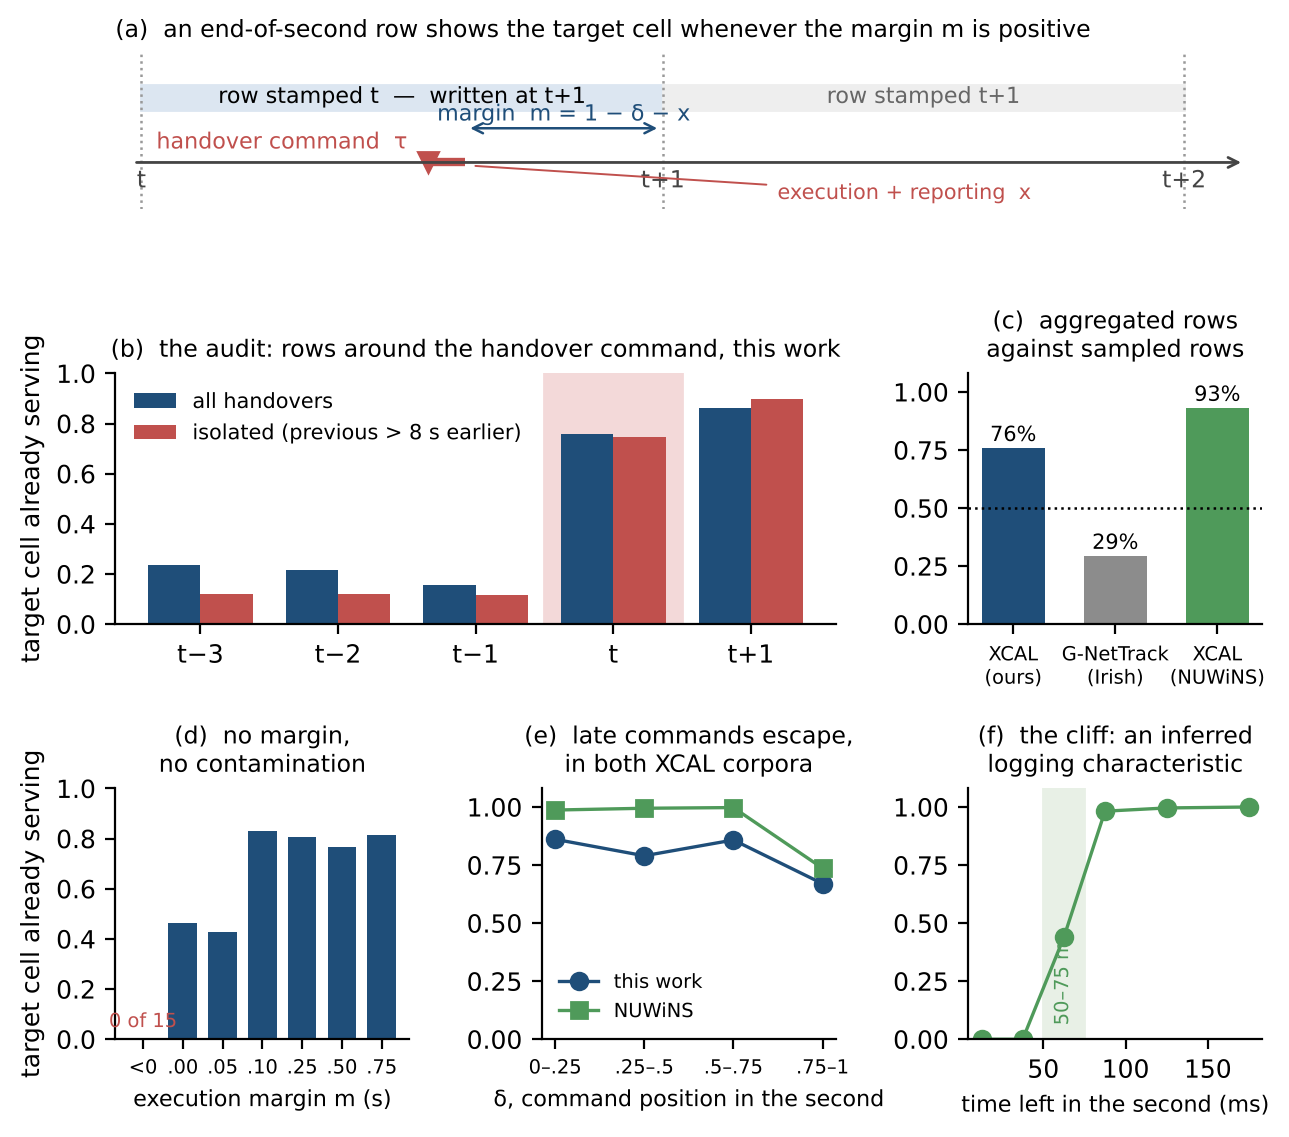
\includegraphics[width=0.84\textwidth]{figures/fig_c9_alignment.png}
\caption{The alignment audit and its mechanism. (a) A command at $\tau$ inside the second $[t,t+1)$ and the margin $m$ of Eq.~\eqref{eq:margin}. (b) Share of handovers whose target already serves in the rows around the command, operator~A. (c) Aggregated against sampled rows: this work, the G-NetTrack traces of~\cite{ref37}, and NUWiNS~\cite{ref40} under an end-of-second rule. (d) Contamination against the margin $m$. (e) Contamination against the command's position $\delta$ in the second, in both XCAL corpora. (f) The contamination cliff near the end of the second, from which a logging characteristic of roughly 60~ms is inferred; it is not a measured latency.}
\label{fig:align}
\end{figure*}

%% =====================================================================
\section{Prediction framework}
\label{sec:framework}

\subsection{Task and hazard formulation}
At each sample $t$ the handset observes features $x_t$; let $T_t$ be the time to the next handover command. The task is the cumulative incidence $F_k(x_t) = P(T_t \le h_k \mid x_t)$ for horizons $h \in \{0.5, 1, 2, 3, 5\}$~s. Fitting one classifier per horizon is free to produce $F_1 > F_2$, an impossible assertion; on our data independent heads violate the ordering on 38.9\% of rows. We therefore partition time into bins $B_k = (h_{k-1}, h_k]$, estimate the discrete-time hazard $\lambda_k(x) = P(T \in B_k \mid T > h_{k-1}, x)$ with a single model over long-format (row, bin) records, and recover
\begin{equation}
F_k(x) = 1 - \prod_{j=1}^{k} \bigl(1 - \lambda_j(x)\bigr),
\label{eq:hazard}
\end{equation}
which is non-decreasing in $k$ for any learner whose output lies in $[0,1]$~\cite{ref48,ref49,ref50}. The case for the formulation is deliberately narrow. Post-hoc projections (a cumulative maximum or pool-adjacent-violators) also reach zero violations, and isotonic calibration~\cite{ref34} composed with them calibrates better if a calibration split can be spared; per-horizon temperature scaling~\cite{ref33} would not preserve the ordering. The hazard model reaches coherence from one fit without a held-out split; its one-second ECE is 0.037 against 0.043 for raw and projected independent heads and 0.015 for the isotonic composite. It does not rank better, and because no retained row is censored inside the horizon grid, its censoring-aware likelihood confers no advantage on this data.

\subsection{Features and alignment}
The main feature set has 112 columns: 89 radio (serving RSRP, RSRQ, SINR, RSSI and CQI; report-projected neighbour RSRP; serving-to-neighbour gaps; rolling means, deviations, ranges and slopes over 3, 5 and 10~s; six missingness masks), 17 mobility (GPS speed, heading change, acceleration, stop state) and 6 history features computed from the decoded signalling clock over the whole session (time since the previous and second-previous command, command counts in the previous 30 and 60~s, whether the previous command was a return). Every export-derived feature is lagged by one row, so that a prediction at $t$ uses only the row closing at or before $t$. Rolling windows are backward-looking, never span a session, and are computed before imputation.

\subsection{Learners}
Seven learners receive the same features, folds, seeds, formulation and tuning budget: logistic regression, LightGBM~\cite{ref32}, a multi-layer perceptron, and three sequence models (GRU, TCN and a Transformer encoder) over windows of the ten most recent lagged feature vectors. Three history-only arms (dwell time, the history block, and exponential-kernel command sums) show what the command stream alone carries. The A3 entry condition is scored as an instantaneous signal-margin proxy with the deployed offsets and hysteresis recovered from signalling; a one-hertz export cannot reproduce the UE's 160--320~ms TTT evaluation or the network's decision, so this is a proxy rather than an emulation of the procedure. LightGBM is the learner carried through the analyses; Section~\ref{sec:blind} shows that this is a convention rather than a finding.

\subsection{Evaluation protocol}
\paragraph{Splitting} The primary protocol is leave-one-campaign-out (LOCO): each campaign is held out in turn, so the test unit is a whole continuous session. Hyper-parameters are chosen by nested random search (20 trials per outer fold) on an internal validation block made of the last 20\% of each training campaign, purged by 60~s; scalers, imputers, thresholds and calibrators are fitted inside the training partition only. Stochastic learners are averaged over three seeds. To measure what the protocol is worth we also run, at fixed hyper-parameters, a ladder of three weaker protocols: contiguous time blocks with a 60~s purge~\cite{ref35}, random 180~s blocks (the protocol this study used before the audit), and random rows (Fig.~\ref{fig:protocols}).

\begin{figure}[t]
\centering
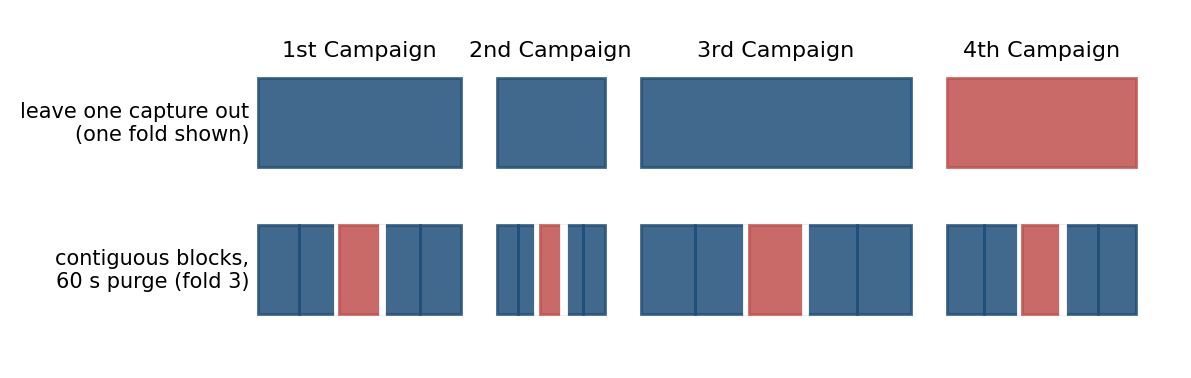
\includegraphics[width=\linewidth]{figures/fig_c1_protocols.png}
\caption{The splitting ladder. Leave-one-campaign-out holds out a whole continuous session; blocked splitting holds out time blocks with a purge; random 180~s blocks and random rows place near-duplicate samples of one session on both sides of the split.}
\label{fig:protocols}
\end{figure}

\paragraph{Metrics} Ranking is reported as AUPRC with its prevalence floor and lift, beside AUROC; calibration as ECE over fifteen equal-mass bins and Brier score; and event-level cost at a 5\% false-positive threshold set on the validation block, as the share of commands detected (a command at $\tau$ is detected at horizon $h$ if a usable row in $[\tau-h,\tau)$ alarms), false-alarm episodes per hour, and median lead time.

\paragraph{Uncertainty} With four independent units, a paired sign test cannot return $p < 0.125$, so no difference is declared significant. We report the observed range over held-out campaigns as the description of between-session variation. Within-session intervals from a block bootstrap over 180~s blocks are given for reference and are anti-conservative, because Section~\ref{sec:ladder} shows those blocks are not independent.

%% =====================================================================
\section{Results}
\label{sec:results}

\subsection{What the leak is worth, and where it lives}
\label{sec:cost}

Table~\ref{tab:cost} holds everything fixed except which columns are shifted by one row: one row set, one learner (LightGBM at fixed hyper-parameters), one set of folds and seeds. Using the row stamped $t$ at $t$ gives a one-second AUPRC of 0.604 and AUROC 0.911; lagging every export column gives 0.157 and 0.744. Read upward, the unaligned score is 3.9 times the aligned one. At five seconds, where one second of misalignment matters less, the change is 0.556 to 0.435. The single-feature effect is starker: serving dwell time computed from the export's serving-cell column reaches AUROC 0.873 on its own, and the same quantity computed from signalling timestamps reaches 0.664.

\begin{table}[t]
\centering
\caption{Lag decomposition. Same rows, folds, seeds and fixed-parameter LightGBM; only the set of columns lagged by one row changes. LOCO, operator~A.}
\label{tab:cost}
\footnotesize
\setlength{\tabcolsep}{3pt}
\begin{tabularx}{\linewidth}{X r c c c}
\toprule
\textbf{Columns lagged} & \textbf{Cols} & \textbf{AUPRC 1 s} & \textbf{AUROC 1 s} & \textbf{AUPRC 5 s} \\
\midrule
None (row $t$ used at $t$) & 0 & 0.604 & 0.911 & 0.556 \\
Neighbour and A3-gap only & 31 & 0.601 & 0.905 & 0.555 \\
Serving-cell radio scalars only & 56 & 0.182 & 0.772 & 0.443 \\
All serving-relative (GPS at $t$) & 92 & 0.156 & 0.743 & 0.435 \\
All export columns (this work) & 109 & 0.157 & 0.744 & 0.435 \\
\midrule
A3 signal-margin proxy & --- & 0.114 & 0.685 & 0.370 \\
\bottomrule
\end{tabularx}
\end{table}

The decomposition locates the leak. Lagging the 31 neighbour and A3-gap columns, the A3 condition itself and the columns an analyst would suspect first, leaves AUPRC at 0.601, under 1\% of the fall. Lagging the 56 serving-cell radio scalars takes it to 0.182, which is 94.4\% of the fall. Lagging the 17 GPS mobility features as well, which no aggregation rule can contaminate, changes it by less than 0.1\%, so the one-row lag costs essentially nothing where it is not needed.

The reason is the part of the finding that transfers to other datasets. A column named \texttt{serving\_rsrp} is not a property of a cell; it is the power of whichever cell the export currently treats as serving. When the assignment flips inside the second, that column silently changes its referent and reports the target's power, which is higher than the source's by construction. The same holds for RSRQ, SINR, CQI and every rolling statistic derived from them. The neighbour gap moves too, but it was already near its trigger threshold, so the flip adds little information. On any export whose rows are aggregates, the columns to distrust are those defined relative to the serving-cell assignment, and they are not the ones that look like identifiers. Within that block the removal of the future cell and one second of feature ageing are confounded on a one-hertz grid, so the lag is a conservative safeguard under the inferred export semantics rather than a measured optimum.

A residual-leak check points the same way. If contamination survived the lag, lift would be highest inside handover bursts, where the next target has just served. It is lowest there: on quiet rows (no command in the previous 10~s) LightGBM reaches AUPRC 0.129 against a 4.3\% floor (3.0\x), and on in-burst rows 0.198 against 11.2\% (1.8\x); the ordering holds for burst cutoffs from 5 to 20~s.

\subsection{The splitting protocol reorders the leaderboard}
\label{sec:ladder}

Table~\ref{tab:ladder} and Fig.~\ref{fig:ladder} hold data, lagged features, formulation, hyper-parameters and seeds fixed and change only the splitting rule. Random-row splitting inflates one-second AUPRC by 49\% for LightGBM, 34\% for the Transformer and 25\% for the GRU, against 8\% for logistic regression and the MLP. Random 180~s blocks, the protocol this study itself used before the audit, still inflate LightGBM by 12\%, because blocks of one continuous session share cells, traffic and trajectory. Contiguous blocks with a 60~s purge remove about half of that and remain 6\% above campaign hold-out; a single-seed sweep keeps them 4--11\% above it for purges of 0 to 180~s. The A3 proxy, which has nothing to fit, moves by 0\% across the ladder, which shows that the inflation is over-fitting to the session rather than a change in test-set difficulty.

\begin{table}[t]
\centering
\caption{One-second AUPRC under four splitting protocols at fixed hyper-parameters (LOCO = leave one campaign out). Last column: inflation of random rows over LOCO.}
\label{tab:ladder}
\footnotesize
\setlength{\tabcolsep}{3pt}
\begin{tabularx}{\linewidth}{X c c c c r}
\toprule
\textbf{Learner} & \textbf{LOCO} & \textbf{\shortstack{Blocks +\\purge}} & \textbf{\shortstack{Random\\180 s}} & \textbf{\shortstack{Random\\rows}} & \textbf{Infl.} \\
\midrule
Logistic regression & 0.165 & 0.163 & 0.168 & 0.178 & +8\% \\
LightGBM & 0.156 & 0.166 & 0.176 & 0.233 & +49\% \\
TCN & 0.154 & 0.146 & 0.158 & 0.174 & +13\% \\
MLP & 0.150 & 0.151 & 0.159 & 0.163 & +8\% \\
Transformer & 0.126 & 0.144 & 0.157 & 0.168 & +34\% \\
GRU & 0.124 & 0.118 & 0.131 & 0.155 & +25\% \\
A3 proxy & 0.114 & 0.114 & 0.114 & 0.114 & +0\% \\
\bottomrule
\end{tabularx}
\end{table}

\begin{figure}[t]
\centering
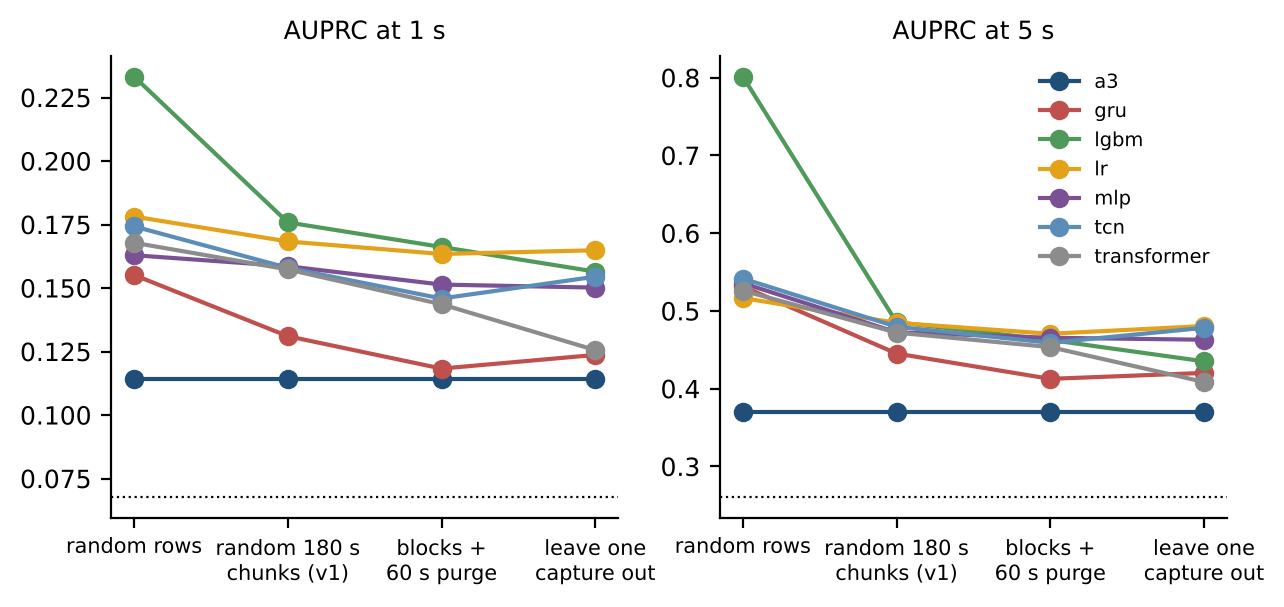
\includegraphics[width=\linewidth]{figures/fig_c2_protocols.png}
\caption{The splitting ladder at one and five seconds, fixed hyper-parameters. The dotted line is the prevalence floor. Random-row splitting inflates LightGBM the most and reverses its rank.}
\label{fig:ladder}
\end{figure}

Because the inflation depends on the architecture, the protocol reorders the leaderboard instead of raising it uniformly. Under campaign hold-out at fixed hyper-parameters the leading learner at one second is logistic regression (0.165); under random rows it is LightGBM (0.233). At five seconds LightGBM moves from fourth under campaign hold-out to first under random rows, inflated by 84\%, while logistic regression falls from first to sixth. A study using random-row splitting, the most common stated protocol in Table~\ref{tab:audit}, would name a different winner on the same data. Section~\ref{sec:blind} shows the same reversal on an unseen operator.

\subsection{The reference level after both repairs}
\label{sec:level}

Table~\ref{tab:level} gives the tuned learners under campaign hold-out with lagged features. At one second LightGBM reaches AUPRC 0.169 against a 6.8\% floor (2.5\x, AUROC 0.773, ECE 0.014); the observed range over the four held-out campaigns is 0.125--0.223, and this range, not the within-session interval, is the honest description of between-session variation. A fifth campaign could fall outside it. At five seconds AUPRC is 0.454 against a 26.1\% floor (1.7\x, range 0.385--0.531). Table~\ref{tab:percamp} gives the per-campaign values. Lift runs from 2.4\x{} to 3.1\x{} and AUROC from 0.768 to 0.797; no single campaign carries the pooled result. The highway campaign has the lowest AUPRC (0.125) but a lift and AUROC inside the urban range, because its prevalence is lowest. On that campaign speed and corridor are collinear (50.9~km/h against 21.4--39.1~km/h), so the difference cannot be attributed to either. The MLP and TCN are within 0.006 of LightGBM at one second and ahead of it at five, so the order of the top arms is not a finding. The best learned models sit above the A3 proxy (0.114) and above the history-only arms (0.105--0.120), so the radio and mobility blocks carry signal beyond the command stream; but the gap between the best learned model and the proxy is smaller than the gap the alignment defect alone produces (Table~\ref{tab:cost}).

\begin{table}[t]
\centering
\caption{Tuned LightGBM at one second, by held-out campaign (operator~A). Every row is exploratory: Campaign~4 is held out from fitting but not blind to the alignment repair.}
\label{tab:percamp}
\footnotesize
\setlength{\tabcolsep}{3pt}
\begin{tabularx}{\linewidth}{X r c c c c c}
\toprule
\textbf{Held out} & \textbf{Rows} & \textbf{Prev.} & \textbf{AUPRC} & \textbf{Lift} & \textbf{AUROC} & \textbf{ECE} \\
\midrule
C1 urban arterial & 2,178 & 8.4\% & 0.199 & 2.4\x & 0.768 & 0.017 \\
C2 urban loop & 1,131 & 8.0\% & 0.223 & 2.8\x & 0.797 & 0.018 \\
C3 dense urban & 3,072 & 6.5\% & 0.198 & 3.1\x & 0.785 & 0.010 \\
C4 highway & 2,205 & 5.1\% & 0.125 & 2.5\x & 0.770 & 0.049 \\
Pooled out of fold & 8,586 & 6.8\% & 0.169 & 2.5\x & 0.773 & 0.014 \\
\bottomrule
\end{tabularx}
\end{table}

\begin{table}[t]
\centering
\caption{Tuned learners, LOCO with lagged features, operator~A. Bracketed: within-session block-bootstrap interval (anti-conservative). LightGBM range over held-out campaigns: 0.125--0.223 (1~s), 0.385--0.531 (5~s).}
\label{tab:level}
\footnotesize
\setlength{\tabcolsep}{2.5pt}
\begin{tabularx}{\linewidth}{X c c c c}
\toprule
\textbf{Learner} & \textbf{AUPRC 1 s} & \textbf{Lift} & \textbf{AUROC} & \textbf{AUPRC 5 s} \\
\midrule
LightGBM & 0.169 [0.150, 0.196] & 2.5\x & 0.773 & 0.454 \\
MLP & 0.168 [0.149, 0.192] & 2.5\x & 0.762 & 0.493 \\
TCN & 0.163 [0.145, 0.189] & 2.4\x & 0.756 & 0.487 \\
Transformer & 0.149 [0.129, 0.179] & 2.2\x & 0.729 & 0.450 \\
GRU & 0.130 [0.117, 0.149] & 1.9\x & 0.702 & 0.449 \\
Kernel history (LR) & 0.120 [0.103, 0.138] & 1.8\x & 0.666 & 0.403 \\
Logistic regression & 0.119 [0.103, 0.143] & 1.8\x & 0.624 & 0.408 \\
A3 proxy & 0.114 [0.101, 0.132] & 1.7\x & 0.685 & 0.370 \\
Dwell time only & 0.105 [0.091, 0.120] & 1.6\x & 0.637 & 0.367 \\
Prevalence floor & 0.068 & 1.0\x & 0.500 & 0.261 \\
\bottomrule
\end{tabularx}
\end{table}

Scored as a warning (Fig.~\ref{fig:events}), the system detects 32.9\% of handover commands at one second, with a median lead of 0.50~s, at 169 false-alarm episodes per hour; at five seconds it detects 43.5\% with a median lead of 3.36~s at 77 per hour. Part of the one-second shortfall is structural: under the 2~s post-handover blanking policy only 64.6\% of commands have any usable row in their one-second lead window. No operating point measured here is deployable for target-cell preparation, which would also require naming the target cell and a lead time long enough to act on, and the lead times are upper bounds because acquisition and inference delays of a live system were not measured.

\begin{figure}[t]
\centering
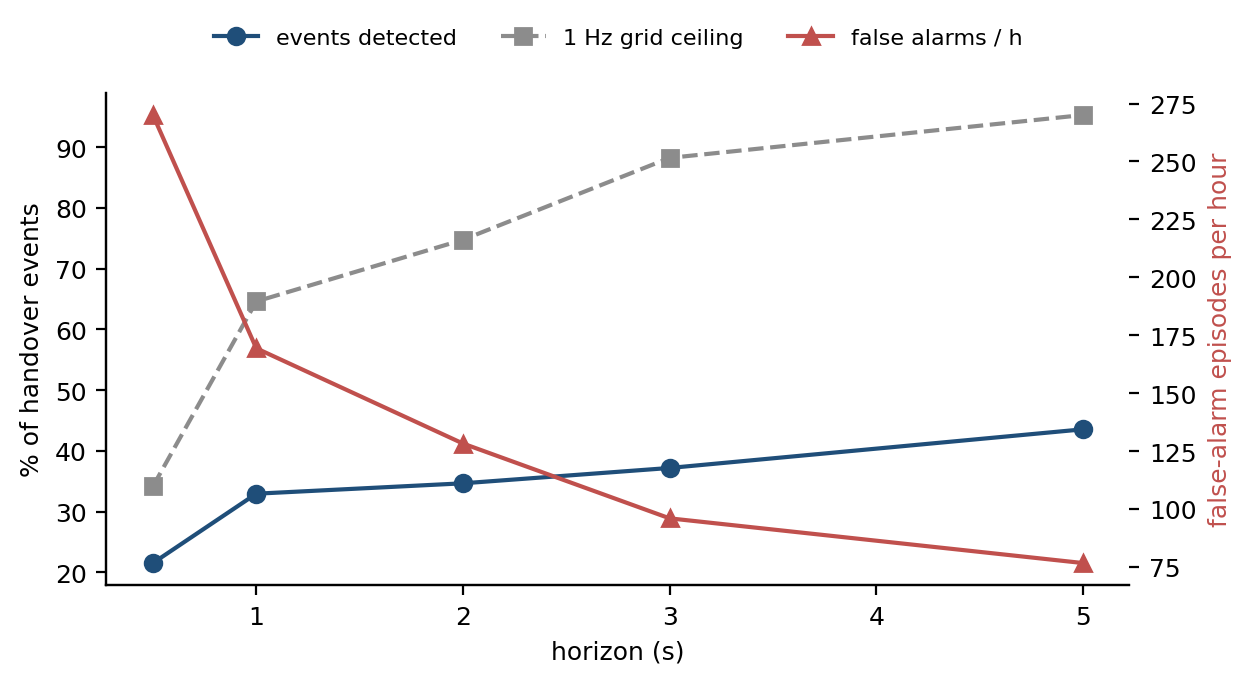
\includegraphics[width=\linewidth]{figures/fig_c18_events.png}
\caption{Event-level cost at the 5\% false-positive threshold, pooled over the four held-out campaigns: share of handover commands detected, share resolvable on the one-hertz grid under 2~s blanking, and false-alarm episodes per hour.}
\label{fig:events}
\end{figure}

\paragraph{Coherence and calibration} Table~\ref{tab:coh} compares the hazard model with independent per-horizon heads and the repairs a reviewer would ask for, all at fixed hyper-parameters on the same folds. Independent heads violate the ordering $F_1 \le \dots \le F_5$ on 38.9\% of rows, by up to 0.43 in probability; per-horizon isotonic calibration makes this worse (44.4\%; Fig.~\ref{fig:coh}). A cumulative maximum or pool-adjacent-violators projection removes every violation at no calibration cost, and so does the hazard model. What separates them is calibration: the hazard model reaches a one-second ECE of 0.037 from one fit without a held-out split, against 0.043 for the free projections, while isotonic calibration followed by a projection reaches 0.015 at the price of a calibration split. Ranking is the same within 0.005 AUPRC for every arm. On a larger corpus the isotonic composite would be the stronger choice; on four sessions, the hazard model is the one that does not spend data.

\begin{table}[t]
\centering
\caption{Coherence and calibration at fixed hyper-parameters, LOCO, operator~A. Viol.: rows on which the horizon ordering is violated (single fit). Split: needs a held-out calibration split.}
\label{tab:coh}
\footnotesize
\setlength{\tabcolsep}{2.5pt}
\begin{tabularx}{\linewidth}{X c c c c c}
\toprule
\textbf{Arm} & \textbf{Viol.} & \textbf{Max} & \textbf{ECE 1 s} & \textbf{AUPRC 1 s} & \textbf{Split} \\
\midrule
Independent heads & 38.9\% & 0.434 & 0.043 & 0.155 & no \\
\quad + cumulative max & 0\% & 0 & 0.043 & 0.156 & no \\
\quad + PAV & 0\% & 0 & 0.043 & 0.155 & no \\
\quad + isotonic & 44.4\% & 0.581 & 0.016 & 0.153 & yes \\
\quad + isotonic + PAV & 0\% & 0 & 0.015 & 0.151 & yes \\
Hazard (this work) & 0\% & 0 & 0.037 & 0.151 & no \\
\bottomrule
\end{tabularx}
\end{table}

\begin{figure}[t]
\centering
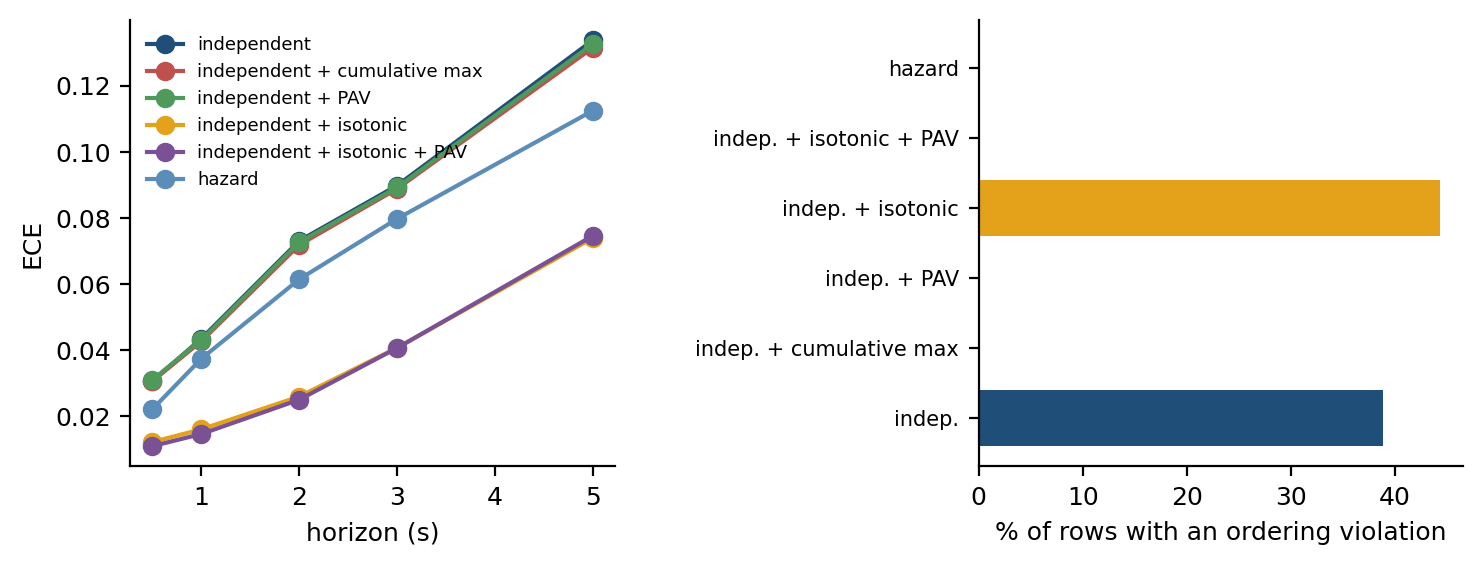
\includegraphics[width=\linewidth]{figures/fig_c11_coherence.png}
\caption{Calibration error by horizon (left) and share of rows violating the horizon ordering (right) for the hazard model, independent per-horizon heads and their repairs; fixed hyper-parameters, LOCO, operator~A.}
\label{fig:coh}
\end{figure}

\paragraph{Conformal risk control} We also examined conformal risk control~\cite{ref21} on the row-level miss loss. Where calibration and test units are exchangeable (half splits of the 57 pooled blocks) it behaves as theory predicts: at $\alpha = 0.20$ the realised loss is 0.171 at a 48\% alarm rate. Across campaigns, which differ by corridor and speed, the guarantee does not apply; the mean loss over the 12 ordered campaign pairs was 0.156, with 8 of 12 at or below $\alpha$, but those rotations are pseudoreplicates of four sessions. We report this as a calibration diagnostic, not an operating guarantee.

\subsection{Blind test on a second operator}
\label{sec:blind}

The operator~B capture differs from the development corpus in ways that matter for mobility (Table~\ref{tab:corpus}): most rows are on Band~40 (TDD), 59\% of handovers change carrier (18--24\% on operator~A), Event~A5 with a 480~ms TTT drives 37\% of handovers, the operator-A profile (A3, +1~dB, 320~ms) is absent, and 98\% of neighbour entries carry RSRP only. The frozen protocol is applied unchanged: fit and calibration rows come from the four operator-A campaigns, hyper-parameters come from the same nested search, results are averaged over three seeds, and only the operator-B rows are scored. This is exactly the fold LOCO would produce for a fifth campaign. Intervals come from a paired bootstrap over eighteen contiguous 60~s segments of the one session and contain no between-session variance.

\paragraph{The leakage findings replicate} The alignment step reappears blind (Table~\ref{tab:align}). The unlagged fixed-parameter model, trained on operator~A, scores AUPRC 0.512 on operator~B against 0.119 lagged, a 4.3-fold inflation against 3.9-fold on operator~A. Neither the audit nor the lag was tuned on this capture, and the lag was fixed before the capture existed.

\paragraph{The level transfers; the ranking does not} Table~\ref{tab:blind} lists every learner. LightGBM reaches 0.137 (2.3\x, AUROC 0.773), inside its operator-A range, but it does not beat the A3 proxy on AUPRC (0.159), though it ranks better (AUROC 0.773 against 0.691). Logistic regression reaches 0.261 (4.4\x, AUROC 0.842) and beats LightGBM by +0.124 [+0.025, +0.208] in the segment bootstrap; the three history-only arms also score above LightGBM, with intervals for the difference that include zero. Calibration separates the learners the other way: logistic regression is poorly calibrated (ECE 0.132), while LightGBM and the history arms stay at or below 0.047.

\begin{table}[t]
\centering
\caption{Blind second-operator test at one second (883 rows, 52 positives, prevalence 5.9\%), trained on operator~A under the frozen protocol. $\Delta$: AUPRC difference against LightGBM, paired bootstrap over eighteen 60~s segments (within-session).}
\label{tab:blind}
\footnotesize
\setlength{\tabcolsep}{2.5pt}
\begin{tabularx}{\linewidth}{X c c c c}
\toprule
\textbf{Learner} & \textbf{AUPRC} & \textbf{AUROC} & \textbf{ECE} & \textbf{$\Delta$ vs LightGBM} \\
\midrule
Logistic regression & 0.261 & 0.842 & 0.132 & +0.124 [+0.025, +0.208] \\
Kernel history (LR) & 0.192 & 0.786 & 0.028 & +0.055 [$-$0.024, +0.085] \\
Dwell time only & 0.190 & 0.792 & 0.030 & +0.053 [$-$0.040, +0.115] \\
History block only & 0.175 & 0.760 & 0.041 & +0.039 [$-$0.031, +0.101] \\
A3 proxy & 0.159 & 0.691 & 0.349 & +0.023 [$-$0.045, +0.053] \\
GRU & 0.144 & 0.787 & 0.037 & --- \\
Transformer & 0.143 & 0.792 & 0.040 & --- \\
LightGBM & 0.137 & 0.773 & 0.047 & --- \\
TCN & 0.136 & 0.775 & 0.046 & --- \\
MLP & 0.135 & 0.767 & 0.058 & $-$0.002 [$-$0.056, +0.044] \\
Prevalence floor & 0.059 & 0.500 & --- & --- \\
\bottomrule
\end{tabularx}
\end{table}

A post-hoc hypothesis, not a result, is that the neighbour and gap features do not mean the same thing on the two networks: operator~B reports RSRP only, configures different offsets and hands over mostly between carriers, so a same-carrier serving-to-neighbour gap says little about an inter-frequency A5 trigger. One observation is consistent with it. In a matched fixed-parameter run, LightGBM scored 0.176 on this capture with the original parser, which recovered 16 of operator~B's 776 neighbour rows, and 0.122 with the corrected parser and the neighbour block present. We do not select a new primary learner on the strength of one 17-minute session, which would repeat on a smaller scale the post-hoc selection this test has just exposed.

%% =====================================================================
\section{Discussion}
\label{sec:discussion}

\subsection{What the findings mean for handover prediction}
The two largest effects in this study come from evaluation choices, not from model choice. A one-row misalignment changes one-second AUPRC by a factor of about four, and the splitting rule by up to 49\%; the spread between the best and worst learned model under a fixed, sound protocol is about 0.04. A reported score on a one-hertz drive-test export therefore says little about a model until two questions are answered: how the export rows are aligned with the event clock, and what unit was held out. Table~\ref{tab:audit} suggests these questions are rarely answered in the recent literature. We do not claim that any audited study is affected; we claim that none provides the information needed to rule it out.

\subsection{Beyond this instrument}
The mechanism is not specific to LTE or to one vendor. Any export that writes one row per interval and stamps it at the interval's start, while filling it with the state at the interval's end, will show the next serving cell before the command whenever the command executes inside the interval. Faster grids shrink the window but do not close it: at 10~Hz, a cell change that completes 60~ms before the row closes still lands in the earlier row. The same reasoning applies to 5G NR handover and conditional handover, to beam switches, and to radio-link-failure labels taken from signalling while features come from an aggregated export. Conversely, tools that sample the modem state at the row timestamp, such as the G-NetTrack traces examined here, should show no aggregation step; the audit distinguishes the two cases in a few lines, so the question can be answered for any dataset that carries an event clock rather than argued from documentation.

\subsection{Recommendations}
The recommendations below are ordered by the size of the effect they guard against on our data. Table~\ref{tab:checklist} restates them as a reporting checklist that an author can complete and a reviewer can check.

\begin{table}[t]
\centering
\caption{Reporting checklist for handover predictors built on drive-test or other aggregated exports, with the effect each item guards against on our data.}
\label{tab:checklist}
\footnotesize
\begin{tabularx}{\linewidth}{X l}
\toprule
\textbf{Report} & \textbf{Effect here} \\
\midrule
Export row semantics, and the alignment audit against the event clock & 3.9--4.3\x \\
Which columns are lagged (serving-relative, not only identifiers) & 94\% of leak \\
The held-out unit (session, route, day), and the per-unit range & +12--49\% \\
History features computed from the signalling clock & AUROC 0.87 vs 0.66 \\
Prevalence floor and lift beside AUPRC; never accuracy alone & floor 6.8\% \\
Calibration (ECE, Brier) and horizon coherence & 38.9\% violations \\
Event-level cost: detection, false alarms per hour, lead time & 33\% @ 169/h \\
A blind capture, and which claims were tested on it & rank reversal \\
\bottomrule
\end{tabularx}
\end{table}

\begin{enumerate}
\item Audit row alignment against decoded signalling before building features (Listing~\ref{lst:audit}). A step at the row stamped before the command flags end-of-second aggregation.
\item If the step is present, lag every export column defined relative to the serving-cell assignment, including radio scalars and their rolling statistics, not only cell identifiers. Compute history features from the signalling clock.
\item Hold out whole sessions or routes, and report the per-session range beside any pooled score. Treat within-session bootstrap intervals as descriptive.
\item Report AUPRC with its prevalence floor, calibration, and event-level costs (detection rate, false alarms per hour, lead time), never accuracy alone on an imbalanced task.
\item Keep at least one capture blind to every pipeline decision, ideally on another network, and test the methodological claims on it before the model ranking.
\end{enumerate}

\subsection{Limitations}
\paragraph{Exploratory development corpus} The repair was derived with all four development campaigns in view, and Campaign~4 is held out only from model fitting. The pipeline thresholds (180~s blocks, 60~s purge, 10~s burst cutoff, 2~s blanking) were chosen during protocol design and were not in the pre-Campaign-4 manifest; a single-seed sensitivity sweep shows local stability around them. Only the operator-B capture is confirmatory, and it is one 17-minute session with 52 positive rows at one second.

\paragraph{Mechanism} The exporter's aggregation rule is inferred from its consequences and from a native-rate public corpus, not documented; within the serving radio block, leak removal and one second of feature ageing cannot be separated at one hertz. All captures used one handset model and one XCAL build, so handset-specific logging and firmware behaviour are untested.

\paragraph{Scope} Four sessions give four independent units, so no difference between learners is tested for significance. Speed and corridor are collinear on the highway campaign. The forecast concerns whether a command occurs, not which cell it names, and the A3 baseline is an instantaneous signal-margin proxy rather than an emulation of the UE's TTT procedure. Labels are completed handover commands; they do not establish that a handover was necessary.

%% =====================================================================
\section{Conclusion}
\label{sec:conclusion}

On one-hertz drive-test exports, the row stamped before a handover command usually already describes the cell the handset is about to join. On our data that single property quadruples the apparent skill of a handover predictor; its cost sits in serving-cell radio scalars that change referent at the flip; end-of-second aggregation of a native-rate trace reproduces it; and it replicates on a second operator that played no part in finding it. With the leak removed and whole sessions held out, the next handover is predictable only modestly, and the ranking of learners depends on the protocol and did not transfer across operators. The audit takes a few lines of code. We recommend it before any predictor built on an aggregated export is trusted, and we release it with the pipeline that produced every number in this paper. Native-rate re-export of these captures, more sessions per operator, and a third operator are the next steps.

%% =====================================================================
\section*{Data and code availability}
The pipeline, the alignment audit, the protocol definitions and the scripts that produce every table in this paper are archived at Zenodo, \url{https://doi.org/10.5281/zenodo.23479562} (frozen release v1.0.0 of \url{https://github.com/SS-Abeer13/Handover-Prediction-Thesis}). The archive also contains the raw one-hertz exports and decoded signalling logs of the five captures, the derived frames, and the tables behind every number reported here.

\section*{CRediT authorship contribution statement}
\textbf{Saadman Sakib:} Conceptualization, Methodology, Software, Investigation, Formal analysis, Writing -- original draft. \textbf{Adhnan Kalim:} Methodology, Investigation, Data curation, Validation, Formal analysis, Writing -- review \& editing. \textbf{Evan Ashfaque:} Investigation, Data curation, Visualization, Writing -- review \& editing. \textbf{Mohammad Tawhid Kawser:} Supervision, Resources, Methodology, Writing -- review \& editing.

\section*{Declaration of competing interest}
One of the authors (M.~T.~Kawser) is a co-author of the public drive-test dataset~\cite{ref38} referred to in Section~\ref{sec:corpus}; that dataset is not used for any result reported here. The authors declare no other competing interests.

\section*{Declaration of generative AI and AI-assisted technologies in the manuscript preparation process}
During the preparation of this work the authors used an AI assistant (Claude, Anthropic) to help condense the thesis on which this article is based into journal form and to edit the language. After using this tool, the authors reviewed and edited the content as needed and take full responsibility for the content of the published article.

\section*{Funding}
This research did not receive any specific grant from funding agencies in the public, commercial, or not-for-profit sectors.

\bibliographystyle{elsarticle-num}
\begin{thebibliography}{54}
\bibitem{ref1} 3GPP, ``Evolved Universal Terrestrial Radio Access (E-UTRA); Radio Resource Control (RRC); Protocol specification,'' 3GPP TS 36.331, Release 17, 2022.

\bibitem{ref7} T. Ankome and E. Hanada, ``Reactive to predictive mobility management: a systematic review of ML-driven handover optimization in 5G and beyond,'' Machine Learning and Knowledge Extraction, vol. 8, no. 5, art. 133, 2026, doi:10.3390/make8050133.

\bibitem{ref8} B. Saoud, I. Shayea, M. A. Alnakhli, and H. Mohamad, ``Mobility and handover management in 5G/6G networks: challenges, innovations, and sustainable solutions,'' Technologies, vol. 13, no. 8, art. 352, 2025, doi:10.3390/technologies13080352.

\bibitem{ref9} C. Chabira, I. Shayea, G. Nurzhaubayeva, L. Aldasheva, D. Yedilkhan, and S. Amanzholova, ``AI-driven handover management and load balancing optimization in ultra-dense 5G/6G cellular networks,'' Technologies, vol. 13, no. 7, art. 276, 2025, doi:10.3390/technologies13070276.

\bibitem{ref54} M. Dzaferagic, B. Missi Xavier, D. Collins, V. D'Onofrio, M. Martinello, and M. Ruffini, ``ML-based handover prediction over a real O-RAN deployment using RAN intelligent controller,'' \textit{IEEE Transactions on Network and Service Management}, vol. 22, no. 1, pp. 635--647, 2025, doi:10.1109/TNSM.2024.3468910.

\bibitem{ref36} S. Kaufman, S. Rosset, C. Perlich, and O. Stitelman, ``Leakage in data mining: formulation, detection, and avoidance,'' ACM Transactions on Knowledge Discovery from Data, vol. 6, no. 4, art. 15, 2012, doi:10.1145/2382577.2382579.

\bibitem{ref56} S. Kapoor and A. Narayanan, ``Leakage and the reproducibility crisis in machine-learning-based science,'' \textit{Patterns}, vol. 4, no. 9, art. 100804, 2023, doi:10.1016/j.patter.2023.100804.

\bibitem{ref3} H. Deng, C. Peng, A. Fida, J. Meng, and Y. C. Hu, ``Mobility support in cellular networks: a measurement study on its configurations and implications,'' in Proc. ACM Internet Measurement Conference (IMC), 2018, doi:10.1145/3278532.3278546.

\bibitem{ref4} M. Ghoshal, I. Khan, P. Dinh, Z. J. Kong, O. Basit, S. Wang, Y. Feng, Y. C. Hu, and D. Koutsonikolas, ``Handover configurations in operational 5G networks: diversity, evolution, and impact on performance,'' arXiv:2511.03116, 2025.

\bibitem{ref5} A. Hassan, A. Narayanan, A. Zhang, W. Ye, R. Zhu, S. Jin, J. Carpenter, Z. M. Mao, F. Qian, and Z.-L. Zhang, ``Vivisecting mobility management in 5G cellular networks,'' in Proc. ACM SIGCOMM, 2022, pp. 86--100, doi:10.1145/3544216.3544217.

\bibitem{ref41} M. Ghoshal, I. Khan, Z. J. Kong, P. Dinh, J. Meng, Y. C. Hu, and D. Koutsonikolas, ``Performance of cellular networks on the wheels,'' in Proc. ACM Internet Measurement Conference (IMC), 2023, doi:10.1145/3618257.3624814.

\bibitem{ref6} Z. Liu, Q. Deng, Z. Tan, Z. Qian, X. Zhang, A. Swami, and S. V. Krishnamurthy, ``M2HO: Mitigating the adverse effects of 5G handovers on TCP,'' in Proc. ACM MobiCom, 2024, doi:10.1145/3636534.3690680.

\bibitem{ref14} D. Zidic, T. Mastelic, I. Nizetic Kosovic, M. Cagalj, and J. Lorincz, ``Analyses of ping-pong handovers in real 4G telecommunication networks,'' Computer Networks, vol. 227, art. 109699, 2023.

\bibitem{ref15} A. Amirova, A. Abdiraman, L. Aldasheva, I. Shayea, D. Yedilkhan, and A. Tussupov, ``Data-driven and machine learning-based analysis of handover behavior and network stability in mobile networks,'' Future Internet, vol. 18, no. 6, art. 290, 2026, doi:10.3390/fi18060290.

\bibitem{ref45} M. Kabeer, R. Nordin, M. Behjati, and S. L. Lau, ``Sequence-based deep learning for handover optimization in dense urban cellular network,'' arXiv:2510.02958, 2025.

\bibitem{ref46} S. V. R. Mandapati, ``Meta-continual mobility forecasting for proactive handover prediction,'' arXiv:2512.11841, 2025.

\bibitem{ref57} P.-H. Chou, D.-C. Lin, H.-Y. Wei, W. Saad, and Y. Tsao, ``Learning-based radio link failure prediction based on measurement dataset in railway environments,'' arXiv:2511.08851, 2026.

\bibitem{ref58} I. Panitsas, A. Mudvari, A. Maatouk, and L. Tassiulas, ``A deep and transfer learning approach for handover management in O-RAN,'' arXiv:2404.08113, 2024 (later versions retitled ``Predictive handover strategy in 6G'').

\bibitem{ref59} K. Boutiba, M. Bagaa, and A. Ksentini, ``Radio link failure prediction in 5G networks,'' in Proc. IEEE Global Communications Conference (GLOBECOM), 2021.

\bibitem{ref60} W.-C. Chien, Y. Huang, B.-Y. Chang, and W.-Y. Hwang, ``Privacy-preserving handover optimization using federated learning and LSTM networks,'' \textit{Sensors}, vol. 24, no. 20, art. 6685, 2024, doi:10.3390/s24206685.

\bibitem{ref61} A. Wadud, F. Golpayegani, and N. Afraz, ``AI-driven multi-modal adaptive handover control optimization for O-RAN,'' arXiv:2603.17158, 2026.

\bibitem{ref62} M. L. A. Bartsioka, A. Giannopoulos, and S. Spantideas, ``Intelligent dynamic handover via AI-assisted signal quality prediction in 6G multi-RAT networks,'' arXiv:2510.14832, 2025.

\bibitem{ref63} K. Sun, Q. Han, Z. Yang, W. Huang, H. Zhang, and V. C. M. Leung, ``Proactive handover type prediction and parameter optimization based on machine learning,'' \textit{IEEE Transactions on Wireless Communications}, vol. 24, no. 4, pp. 3515--3528, 2025, doi:10.1109/TWC.2025.3531702.

\bibitem{ref64} A. Gonzalez Bermudez, M. Farreras, M. Groshev, J. A. Trujillo, I. de la Bandera, and R. Barco, ``Graph neural networks for O-RAN mobility management: a link prediction approach,'' arXiv:2502.02170, 2025.

\bibitem{ref65} K. Hasan, T. Trappenberg, and I. Haque, ``A generalized transformer-based radio link failure prediction framework in 5G RANs,'' arXiv:2407.05197, 2024.

\bibitem{ref66} M. Santana and K. L. Dias, ``Open RAN-enabled deep learning-assisted mobility management for connected vehicles,'' arXiv:2412.21161, 2024.

\bibitem{ref67} M. V. Narayana, R. Singh, M. R. Deepa, and R. K. Ganti, ``Enabling AI-native mobility in 6G: a real-world dataset for handover, beam management, and timing advance,'' arXiv:2605.12453, 2026.

\bibitem{ref68} S. Wu, M. Alrabeiah, A. Hredzak, C. Chakrabarti, and A. Alkhateeb, ``Deep learning for moving blockage prediction using real millimeter wave measurements,'' in Proc. IEEE International Conference on Communications (ICC), 2022, arXiv:2101.06886.

\bibitem{ref69} C. Lee, H. Cho, S. Song, and J.-M. Chung, ``Prediction-based conditional handover for 5G mm-wave networks: a deep-learning approach,'' \textit{IEEE Vehicular Technology Magazine}, vol. 15, no. 1, pp. 54--62, 2020, doi:10.1109/MVT.2019.2959065.

\bibitem{ref70} I. A. Safiullin, I. P. Ashaev, A. A. Korobkov, A. K. Gaysin, and A. F. Nadeev, ``Reinforcement learning-based handover algorithm for 5G/6G AI-RAN,'' \textit{Inventions}, vol. 11, no. 1, art. 8, 2026, doi:10.3390/inventions11010008.

\bibitem{ref35} D. R. Roberts et al., ``Cross-validation strategies for data with temporal, spatial, hierarchical, or phylogenetic structure,'' Ecography, vol. 40, no. 8, pp. 913--929, 2017, doi:10.1111/ecog.02881.

\bibitem{ref42} D. Hong and S. S. Rappaport, ``Traffic model and performance analysis for cellular mobile radio telephone systems with prioritized and nonprioritized handoff procedures,'' IEEE Transactions on Vehicular Technology, vol. 35, no. 3, pp. 77--92, 1986.

\bibitem{ref43} X. Lin, R. K. Ganti, P. J. Fleming, and J. G. Andrews, ``Towards understanding the fundamentals of mobility in cellular networks,'' IEEE Transactions on Wireless Communications, vol. 12, no. 4, pp. 1686--1698, Apr. 2013, doi:10.1109/TWC.2013.022113.120512.

\bibitem{ref44} S. Sadr and R. S. Adve, ``Handoff rate and coverage analysis in multi-tier heterogeneous networks,'' IEEE Transactions on Wireless Communications, vol. 14, no. 5, pp. 2626--2638, May 2015, doi:10.1109/TWC.2015.2390231.

\bibitem{ref48} R. L. Prentice and L. A. Gloeckler, ``Regression analysis of grouped survival data with application to breast cancer data,'' Biometrics, vol. 34, no. 1, pp. 57--67, 1978, doi:10.2307/2529588.

\bibitem{ref49} P. D. Allison, ``Discrete-time methods for the analysis of event histories,'' Sociological Methodology, vol. 13, pp. 61--98, 1982, doi:10.2307/270718.

\bibitem{ref50} G. Tutz and M. Schmid, \textit{Modeling Discrete Time-to-Event Data}, Springer Series in Statistics, Springer, Cham, 2016, doi:10.1007/978-3-319-31552-2.

\bibitem{ref16} S. Wiegrebe, P. Kopper, R. Sonabend, B. Bischl, and A. Bender, ``Deep learning for survival analysis: a review,'' Artificial Intelligence Review, vol. 57, no. 3, art. 65, 2024, doi:10.1007/s10462-023-10681-3.

\bibitem{ref17} H.-C. Thorsen-Meyer, D. Placido, B. S. Kaas-Hansen, et al., ``Discrete-time survival analysis in the critically ill: a deep learning approach using heterogeneous data,'' npj Digital Medicine, vol. 5, art. 142, 2022, doi:10.1038/s41746-022-00679-6.

\bibitem{ref18} E. J. Cand\`es, L. Lei, and Z. Ren, ``Conformalized survival analysis,'' Journal of the Royal Statistical Society Series B, vol. 85, no. 1, pp. 24--45, 2023, doi:10.1093/jrsssb/qkac004.

\bibitem{ref21} A. N. Angelopoulos, S. Bates, A. Fisch, L. Lei, and T. Schuster, ``Conformal risk control,'' in Proc. International Conference on Learning Representations (ICLR), 2024.

\bibitem{ref22} S. Bates, A. Angelopoulos, L. Lei, J. Malik, and M. I. Jordan, ``Distribution-free, risk-controlling prediction sets,'' Journal of the ACM, vol. 68, no. 6, 2021, doi:10.1145/3478535.

\bibitem{ref19} K. M. Cohen, S. Park, O. Simeone, and S. Shamai (Shitz), ``Calibrating AI models for wireless communications via conformal prediction,'' arXiv:2212.07775, 2022.

\bibitem{ref20} O. Simeone, S. Park, and M. Zecchin, ``Conformal calibration: ensuring the reliability of black-box AI in wireless systems,'' arXiv:2504.09310, 2025.

\bibitem{ref55} K. Rezaei, M. Sattari, J. Aliakbari, T. Svensson, P. Monti, and C. Natalino, ``TRACE-CRC: trajectory-adaptive conformal risk control for multi-step channel state information prediction,'' in \textit{Proc. Symposium on Conformal and Probabilistic Prediction with Applications}, PMLR vol. 329, pp. 984--1009, 2026.

\bibitem{ref51} R. J. Tibshirani, R. Foygel Barber, E. Cand\`es, and A. Ramdas, ``Conformal prediction under covariate shift,'' in \textit{Advances in Neural Information Processing Systems 32 (NeurIPS)}, 2019, pp. 2530--2540.

\bibitem{ref52} R. Foygel Barber, E. J. Cand\`es, A. Ramdas, and R. J. Tibshirani, ``Conformal prediction beyond exchangeability,'' \textit{The Annals of Statistics}, vol. 51, no. 2, pp. 816--845, 2023, doi:10.1214/23-AOS2276.

\bibitem{ref53} I. Gibbs and E. Cand\`es, ``Adaptive conformal inference under distribution shift,'' in \textit{Advances in Neural Information Processing Systems 34 (NeurIPS)}, 2021, pp. 1660--1672.

\bibitem{ref38} M. M. S. Shafi, K. M. Istiaque, S. S. Sowad, and M. T. Kawser, ``Drive-test-based LTE handover dataset for cellular mobility studies in urban Bangladesh,'' Mendeley Data, version 2, 2025, doi:10.17632/n2pvmtyn2j.2.

\bibitem{ref40} F. Chen, M. Ghoshal, E. Nan, P. Dinh, I. Khan, Z. J. Kong, Y. C. Hu, and D. Koutsonikolas, ``A large-scale study of the potential of multi-carrier access in the 5G era,'' in Passive and Active Measurement (PAM), LNCS vol. 15567, 2025, pp. 469--484, doi:10.1007/978-3-031-85960-1\_19. Dataset: github.com/NUWiNS/pam2025-multi-carrier-dataset.

\bibitem{ref37} D. Raca, D. Leahy, C. J. Sreenan, and J. J. Quinlan, ``Beyond throughput, the next generation: a 5G dataset with channel and context metrics,'' in Proc. ACM Multimedia Systems Conference (MMSys), 2020, pp. 303--308, doi:10.1145/3339825.3394938. Dataset: github.com/uccmisl/5Gdataset (GPL-3.0).

\bibitem{ref34} B. Zadrozny and C. Elkan, ``Transforming classifier scores into accurate multiclass probability estimates,'' in Proc. ACM SIGKDD, 2002, pp. 694--699.

\bibitem{ref33} C. Guo, G. Pleiss, Y. Sun, and K. Q. Weinberger, ``On calibration of modern neural networks,'' in Proc. ICML, 2017, pp. 1321--1330.

\bibitem{ref32} G. Ke, Q. Meng, T. Finley, T. Wang, W. Chen, W. Ma, Q. Ye, and T.-Y. Liu, ``LightGBM: a highly efficient gradient boosting decision tree,'' in Advances in Neural Information Processing Systems 30, 2017, pp. 3146--3154.

\end{thebibliography}


\end{document}
